\documentclass{pre-tfg}

\usepackage{listings}
\usepackage{formular}
\usepackage[pdftex]{graphicx}
\usepackage{hyperref}
\usepackage{todonotes}

\showhelp  % comenta o borra para eliminar ayudas

\title{(TITLE)}
\author{María González Gutiérrez}
\docdate{(MONTH)}{(2020)}


\DeclareGraphicsExtensions{.pdf,.png,.jpg}

\usepackage{color}
\definecolor{gray97}{gray}{.97}
\definecolor{gray75}{gray}{.75}
\definecolor{gray45}{gray}{.45}

\lstset{ frame=Ltb,
     framerule=0pt,
     aboveskip=0.5cm,
     framextopmargin=3pt,
     framexbottommargin=3pt,
     framexleftmargin=0.4cm,
     framesep=0pt,
     rulesep=.4pt,
     backgroundcolor=\color{gray97},
     rulesepcolor=\color{black},
     %
     stringstyle=\ttfamily,
     showstringspaces = false,
     basicstyle=\small\ttfamily,
     commentstyle=\color{gray45},
     keywordstyle=\bfseries,
     %
     numbers=left,
     numbersep=15pt,
     numberstyle=\tiny,
     numberfirstline = false,
     breaklines=true,
   }

% minimizar fragmentado de listados
\lstnewenvironment{listing}[1][]
   {\lstset{#1}\pagebreak[0]}{\pagebreak[0]}

\lstdefinestyle{consola}
   {basicstyle=\scriptsize\bf\ttfamily,
    backgroundcolor=\color{gray75},
   }

\lstdefinestyle{C}
   {language=C,
   }


\renewcommand*\lstlistingname{Listado}



\begin{document}

\maketitle
\tableofcontents

\newpage


\section{INTRODUCCIÓN Y OBJETIVOS}


\section{FANFICTION, WEB ARCHIVE OF OUR OWN Y RELATOS A UTILIZAR}
Un fanfic (abreviatura de “fanfiction”, “ficción del fan”) es una historia basada en una historia ya existente. Son, en esencia, historias creadas sin ánimo de lucro por los fans de un libro, película o videojuego. 
Crear fanfiction, en general, consiste en explorar temas e ideas que uno siente que faltan en la historia original. Puesto que cada fan tiene una interpretación distinta de los personajes y el mensaje que la historia original transmite, el fan convertido en autor puede añadir o quitar a la historia original lo que considere oportuno para contar su propia visión. Esto significa que cada fanfic es efectivamente una “transformación” de la historia original.
El fanfic cae en una zona gris en términos de derechos de autor, pero suele considerarse “fair use”. A día de hoy, la mayoría de fanfics se publican en sitios web de toda índole, destacando entre ellos \href{archiveofourown.org}{Archive Of Our Own}, que es un archivo open-source y sin ánimo de lucro creado expresamente para alojar obras creadas por fans. Según sus datos de mayo de 2020, tiene más de dos millones de usuarios registrados y más de seis millones de trabajos alojados. En particular elegí descargar los fanfics basados en \textit{Good Omens}, un libro de Terry Pratchett y Neil Gaiman, tanto por la cantidad de relatos existente como por mi familiaridad con esa comunidad.

Además de la cantidad y variedad de relatos que aloja, los motivos por el que elegí extraer los datos de Archive Of Our Own son su herramienta de búsqueda y filtrado, su sistema de etiquetas y el hecho de que permite descargar el archivo en HTML. Archive Of Our Own permite filtrar fanfics según varios parámetros y genera un enlace a ese subconjunto de relatos particular, muy útil para descargar una gran cantidad de datos.


\section{RECOGIDA DE FANFICS USANDO LA BASE DE DATOS DE ARCHIVE OF OUR OWN}

En el momento en el que decidí utilizar los fanfics de \textit{Good Omens} para el proyecto, dicho libro tenía unos 22000 fanfics en \href{archiveofourown.org}{Archive Of Our Own} (AO3 para abreviar). Sin embargo, de todos esos relatos sólo me interesaban los que están en inglés y los que realmente contuvieran texto (puesto que, aunque AO3 se centra en texto, permite todo tipo de archivos multimedia), de modo que utilicé el sistema de filtrado del sitio para seleccionar sólo los fanfics en inglés y que no estuvieran etiquetadas como "fanart", "podfic", etc, ya que indican que la obra no tiene texto. Tras este filtrado, quedaron 20190 relatos.

AO3 crea un enlace que lleva siempre a ese subconjunto de relatos, al cual puedo enviar peticiones HTTP GET y navegar las páginas. Cada página contiene un máximo de 20 fanfics, y antes de descargarlos es necesario llevar a cabo un segundo filtrado para evitar las obras sin texto que no hayan sido etiquetadas como tal por su autor. Decidí crear dos \textit{scrapers} distintos, uno para navegar por las páginas, filtrar y guardar los \textit{links} en un archivo, y otro que simplemente lee dicho archivo y realiza descargas.

\begin{itemize}
	\item El primer \textit{scraper} envía peticiones a AO3, explora el HTML de cada página para encontrar los objetos que encapsulan la información de cada fanfic, selecciona aquellos que tengan al menos 40 palabras por capítulo y crea una lista con los enlaces, que guarda en un archivo \textit{txt}.
	\item El segundo \textit{scraper} recorre los enlaces de dicho archivo y los descarga en una carpeta del sistema. Está hecho de tal manera que se le puede indicar qué tramo de la lista tiene que descargar (por ejemplo, del número 5000 al 6000).
	
\end{itemize}

Ambos \textit{scrapers} se encontraban de vez en cuando con el error 429 (Too Many Requests) y el 404 (Page Not Found). Se capturan fácilmente con un \textit{try-catch} que detecta el status de la página; para el 429 simplemente lanza una espera de dos minutos tras la cual reanuda su ejecución por donde la dejó, y para el 404 simplemente pasa a la siguiente, pues este error indica que el autor ha borrado su obra de la página y ya no está accesible.
 
Decidí dividir este proceso en dos programas (el de navegación y filtrado, y el que únicamente descarga) en vez de hacerlo todo en uno porque descargar los más de 20000 archivos de una vez lógicamente tardaría varias horas, y pensé que sería más pragmático si ejecuto una vez el \textit{scraper} crea una lista de enlaces, y luego ya ejecuto todas las veces que sean necesarias el \textit{scraper} que descarga, descargando cada vez un tramo distinto de la lista. De esta forma, pude descargar todos los fanfics en grupos de 2000 (alrededor de una hora y media), pudiendo tener el ordenador libre el resto del tiempo.

El poder ejecutar varias veces el segundo \textit{scraper} sin tener que volver a empezar desde el principio también demostró ser útil para lidiar con errores de red.

Ambos \textit{scrapers} utilizan la librería bs4 y BeautifulSoup para descargar y manejar los archivos HTTP. El resultado de su ejecución es una carpeta con 818,8 MB de archivos HTML.

\section{LIMPIEZA DE DATOS}

\section{ALGORITMO DE IDENTIFICACIÓN DE ENTIDADES}

\section{RECOMENDACIONES}

Aquí habría que insertar tantas secciones como el alumno considere.

A continuación se indican una serie de recomendaciones que seguidas mejorarán la calificación final del trabajo.

\begin{itemize}
 \item Agrupar párrafos. La división del texto en múltiples párrafos independientes de pequeña longitud dificulta la lectura continua del documento.
\item  Evitar abusar de las listas con viñetas y las enumeraciones.
\item Utilizar un máximo nivel de profundidad secciones de 3 (hasta 3.1.1). Si se hace necesario una división más baja, no hacerlo con enumeración de subsecciones sino con texto en negrita y/o subrayada que represente el comienzo de cada subsección. 
\item  Si no hay más de una sección en un nivel no crearla. Es decir, si no hay al menos una 3.2 no crear la 3.1, ya que no tendría sentido dividir la sección 3.
\item  Utilizar referencias absolutas numéricas a tablas, figuras, secciones, etc. Por ejemplo: en la "Figura 3, se muestra el gráfico que  ..."; "Los resultados finales se encuentran en la Tabla X". Usar los ref y labels para que se actualicen las numeraciones automáticamente. No se debe hablar de ``en la siguiente figura'', ¿Qué pasa si reordeamos el texto o lo hace látex de manera automática?.
\item Cuando se referencia a una tabla, figura, sección, etc. hacerlo con la primera letra en mayúscula, ``En la Sección 1 ...''
\item  El texto siempre debe tener una alineación justificada. 
\item En el inicio de cada sección se debe hacer una breve introducción de lo que contiene y al final, unas pequeñas conclusiones y si es posible un texto de pequeña longitud que una con el siguiente capítulo.
\end{itemize}


\subsection{Inserción de Imágenes}

\begin{figure}[!h]
\centering
   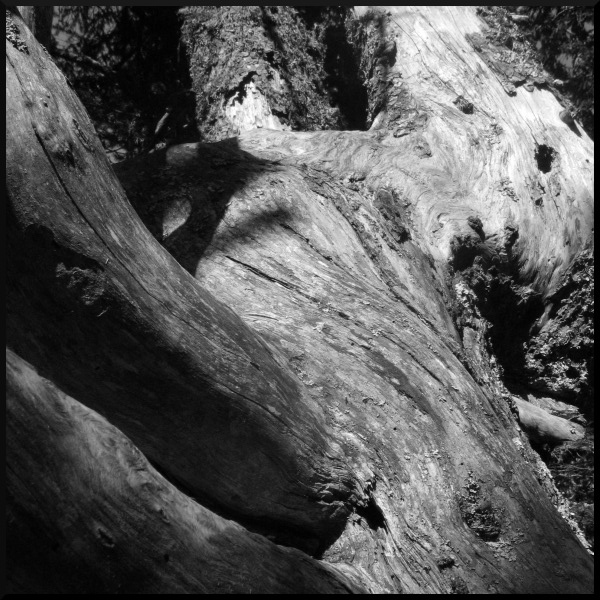
\includegraphics[width=8cm]{figures/tree04.jpg}
\caption{Árbol antiguo}
\end{figure}

\subsection{Inserción de órdenes de línea de comandos}

\begin{listing}[style=consola, numbers=none]
 gcc  -o e21 e21.c
\end{listing}





\subsection{Inserción de Código}

\begin{lstlisting}[caption=Ejemplo de código,style=C]

##include <stdio.h>
#include <sys/types.h>
#include <unistd.h>
#include <stdlib.h>

int main(void){

int register i;
int numHijos=4;
pid_t childpid;

for (i=0;i<numHijos;i++)
  if (childpid=fork()==0){
    sleep(1);
    printf("Proceso %ld con padre %ld\n", (long)getpid(), (long)getppid());
    exit(0);
  }

printf("Soy el proceso padre %ld\n", (long)getpid());
return 0;
}
\end{lstlisting}




\section{MEDIOS QUE SE PRETENDEN UTILIZAR}

\subsection{Medios Hardware}

El alumno deberá describir los medios hardware que prevé serán necesarios para el
desarrollo del proyecto.


\subsection{Medios Software}

El alumno deberá describir los medios software (lenguajes, entornos de desarrollo,
herramientas de gestión y planificación, etc.) que prevé serán necesarios para el
desarrollo del proyecto


\section{REFERENCIAS}

En esta sección se incluirán todas las referencias bibliográficas, ordenadas
alfabéticamente por el primer apellido del primer autor, de las obras de las cuales se
haya realizado alguna cita en los apartados anteriores. Las referencias deberán contener
datos básicos como nombre y apellidos de los autores, título de la obra, evento al que
pertenece, páginas, fecha y lugar de celebración (si se tratara de artículos de congreso),
ISBN, editorial y ciudad (si se tratara de libro), nombre de revista, páginas, volumen y
número (si se tratara de revista), etc.

Se empleará un formato de referencia reconocido en el ámbito académico como
ACM\footnote{http://www.acm.org/sigs/publications/proceedings-templates}\footnote{http://www.cs.ucy.ac.cy/\~{}chryssis/specs/ACM-refguide.pdf}.
Otros formatos aconsejables son, por ejemplo, IEEE, AMA, APA y AMA.

A continuación una sección de «Referencias» con ejemplos de referencias con formato ACM para:

\begin{itemize}
\item Un artículo de revista~\cite{Bow93}.
\item Un informe técnico~\cite{Ding97}.
\item Un libro~\cite{Tavel07}.
\item Un capítulo de libro~\cite{Greiner99}.
\item Un artículo en las actas de un congreso~\cite{Frohlic00}.
\item Para una página web~\cite{Steele04} (con autores conocidos).
\item Para una página web~\cite{Oxygen} (con autores desconocidos).
\end{itemize}


\bibliographystyle{alpha}
\singlespacing
\bibliography{ejemplo}


\end{document}


% Local Variables:
% coding: utf-8
% mode: flyspell
% ispell-local-dictionary: "castellano8"
% mode: latex
% End:
